\item O projétil de massa \SI{3}{\kilogram} é disparado de um canhão a uma velocidade na boca do canhão $v_{0}=\SI{500}{\meter/\second}$. Determine a quantidade de movimento angular do projétil em relação ao ponto $O$ no instante que ele está na altura máxima de sua trajetória.

\import{sections/answers/}{answer-14}

\vspace{-1.6cm}
\begin{flushright}
	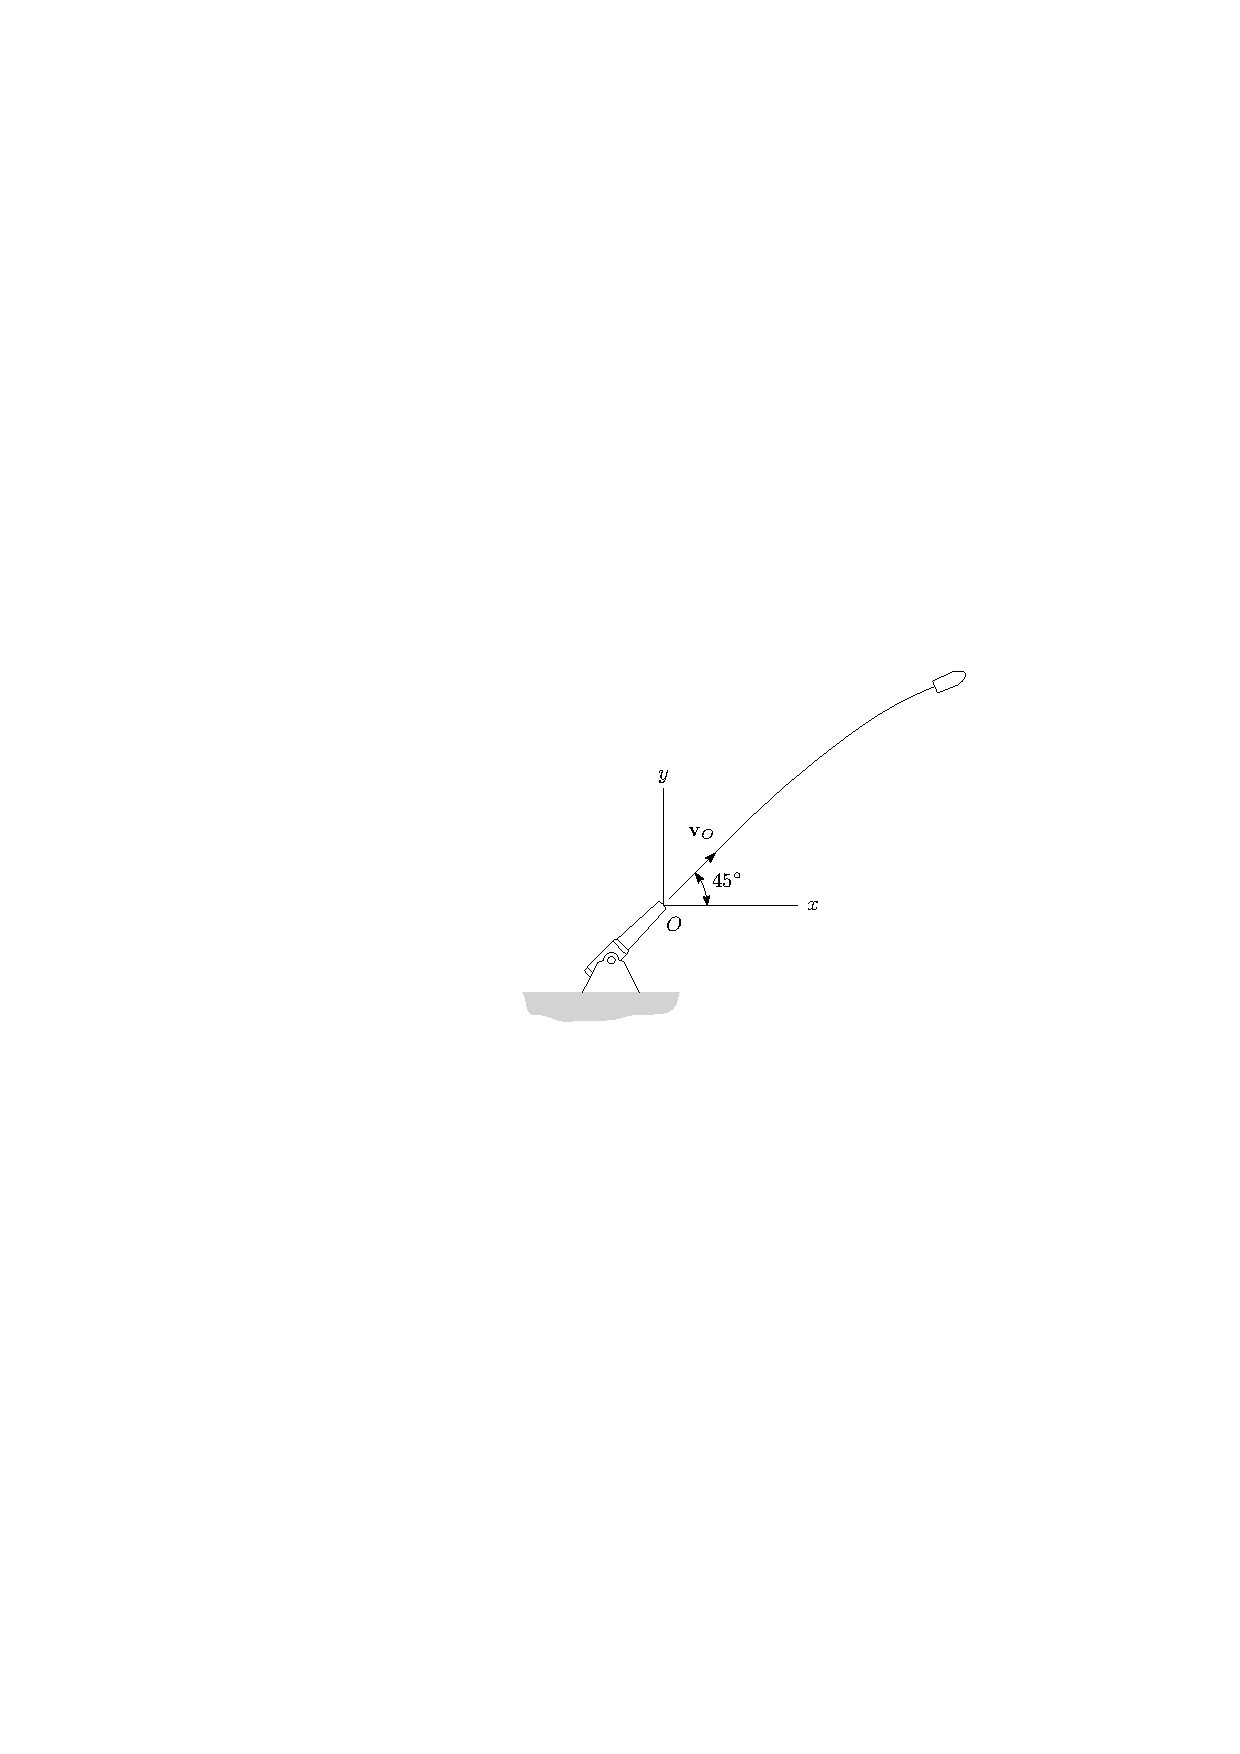
\includegraphics[scale=1.3]{images/draw_6}
\end{flushright}